\documentclass[twoside]{article}
\input{ISC18-english.sty}
%%%%%%%%%%%%%%%%%%%%%%%%%%%%  Make sure to compile twice for proper cross-references. %%%%%%%%%%%%%%%%%%%%%%%
%%%%%%% For proper display of references, compile the document twice. %%%%%%%%%%%%%%%%%%%%% 
%%%%%%%%%%%%%%% If using TeX Live, compile using pdflatex command %%%%%%%%%%%%%%%%%%%%%%%
\begin{document}
\thispagestyle{empty}
%%%%%%%%%%%%%%%%% Article title header  %%%%%%%%%%%%%%%%%%%%
\fancyhead[LE]{Entropy in Inflated Count Data: A Comparative Analysis}
%%%%%%%%%%%%%%%%% Article authors header   %%%%%%%%%%%%%%%%%%%%
%\fancyhead[RO]{Farhadian, R. and Lorvand, H.}
\begin{center}
{
\includegraphics [height=25mm, width=150.3mm] {Images/isc18E}} \\
\vspace*{-1.8cm}
%\begin{center}
%\color{blue} 
%{\hspace{0.1cm}\rule{\textwidth}{1mm}}\\
%\end{center}
\vspace*{4cm}
%%%%%%%%%%%%%%%%% Article title  %%%%%%%%%%%%%%%%%%%%
{\Large \bf Entropy in Inflated Count Data: A Comparative Analysis}\\
%%%%%%%%%%%%%%%%% Article authors and affiliations %%%%%%%%%%%%%%%%%%%%
{\bf
Reza Farhadian  \footnote[1]{{\bf Corresponding Author:} {\tt farhadian.reza@yahoo.com }}, Hamed Lorvand $^2$ \\
$^1$Department of Statistics, Razi University, Kermanshah, Iran\\
$^2$Department of Mathematical Sciences, Isfahan University of Technology, Isfahan, 84156-83111, Iran}
\end{center}
\rule{\textwidth}{0.2mm}\\
%%%%%%%%%%%%%%%%% Article abstract  %%%%%%%%%%%%%%%%%%%%
\noindent{\bf Abstract:}\\
Entropy is a fundamental measure of uncertainty in random variables and depends on the underlying probability distribution. Consequently, even small changes in the probability mass assigned to observed values may substantially affect the entropy. In this paper, we study the entropy of count data under an inflated distribution and present a theorem comparing the entropy of the inflated model with that of the corresponding regular distribution.
 
\noindent{\bf Keywords:} 
Count data, Inflated distribution, entropy. \\  
\noindent{\bf Mathematics Subject Classification (2010):} $\rm 94A17$, $\rm 60E05$. \\
\hspace{1cm}\rule{\textwidth}{0.2mm}
%%%%%%%%%%%%%%
\section{Introduction}
In the mathematical theory of communication, a common quantity for measuring the information content of data is the \textit{entropy measure}. Entropy is a measure of the expected amount of information in some data, and for a random variable $X$ with probability mass function (PMF) $p(x)=\Pr(X=x)$, is calculated by 
\begin{eqnarray*}
	H(X)=-\sum_{x}p(x)\ln p(x).
\end{eqnarray*}

Indeed, entropy is the average amount of information required to determine the outcome of a random variable. On this basis, it may also be interpreted as uncertainty of outcome. Therefore,
this measure is useful for comparing the uncertainty between two random variables such that if the entropy of one of the random variables is less than the other, then its uncertainty is also less. 


Historically, the entropy measure based on the probabilities of random variables was first formulated by Shannon in 1948 (see \cite{Shannon}). However, twenty years before Shannon, Hartley in 1928 pointed out that a phenomenon can contain information if it has multiple possible outcomes \cite{Hartley}. This facilitated the application of the concept of entropy to a random variable. For more information on entropy, see \cite{Brookes}.

It is clear that even small changes in the probabilities of possible values ​​of a random variable can cause significant changes in entropy.
Therefore, it is important to understand how the direction of changes in entropy occurs relative to the type of changes in probabilities.

In this paper, we are interested in investigating the effect of increasing the probability at some specific points from the support of an integer-valued random variable, which represents the concept of \textit{inflation}, and its effect on entropy. To this end, in subsequent sections, we will first give a brief introduction to inflated distributions and then prove the main results related to entropy.

\section{Inflated distribution}
In the data analysis, selecting an appropriate statistical distribution is one of the important tasks. Statistical modeling is rapidly growing in  different sciences due to the development of technological advances and variety of data. 
Hence, modeling count variables is widely used in sciences such as biology, ecology, sociology, epidemiology, engineering, etc. 
For example, count data in everyday medical practice include the numbers of patients arriving in an emergency room between certain hours, phone calls received by an emergency call center in a day, the number of heart attacks, the number of depressive symptoms that a child exhibits, and the number of cigarettes smoked by adolescents. 


It may happen that in the count data, there is an excess number of frequencies at a particular count.  When the frequency of a particular variable is significantly higher than the one predicted by a usual probability distribution, then we are dealing with inflation, and in this case, the \textit{inflated distribution} is used, which is a mixture between a probability distribution to a point mass at a particular count and any other count distribution supported by non-negative integers.
In general, a random variable $Y$ is said to be an inflated distribution
if its PMF is given by
\begin{equation}\label{1}
	\Pr(Y=y)=\begin{cases}
		\alpha+(1-\alpha)\Pr(X=\delta) & \text{if $y=\delta$},\\
		(1-\alpha)\Pr(X=y)& \text{if $y\in\{0, 1, \dots, \delta-1, \delta+1, \dots\}$},
	\end{cases}
\end{equation}
where $\delta$ is the point at which the distribution is inflated, $\alpha\in[0,1]$ is an inflation parameter, and $\Pr(X=x)$ is a regular PMF of count data $X$. 


It can be easily shown that the probability of occurrence of $\delta$ in an inflated distribution is greater than that in a distribution with the regular PMF $P(X=x)$, namely,
\begin{align*}
	\Pr(Y=\delta)=\alpha+(1-\alpha)\Pr(X=\delta)=\Pr(X=\delta)+\alpha(1-\Pr(X=\delta))
	\geq \Pr(X=\delta).
\end{align*}


There are various examples of inflated distribution in Eq. \eqref{1} for particular values of $\delta$ and some common probability distribution for count data. For $\delta=0$, we have zero-inflated models that are very popular in many areas of science.  For instance, zero-inflated Poisson (ZIP) distribution (\cite{Cohen} and \cite{Lambert}) is one of the most popular examples of zero-inflated distributions. The PMF of ZIP is given by
\begin{equation*}
	\Pr(Y=y)=\begin{cases}
		\alpha+(1-\alpha)e^{-\lambda} & \text{if $y=0$},\\
		(1-\alpha)\frac{\lambda^ye^{-\lambda}}{y!}& \text{if $y=1, 2, \dots$},
	\end{cases}\qquad (\lambda>0).
\end{equation*}

 Figure \ref{F} depicts the histograms of the Poisson and ZIP distributions for different choices of parameters $\alpha$ and $\lambda$. 
 
\begin{figure}[htb] 
	\centerline{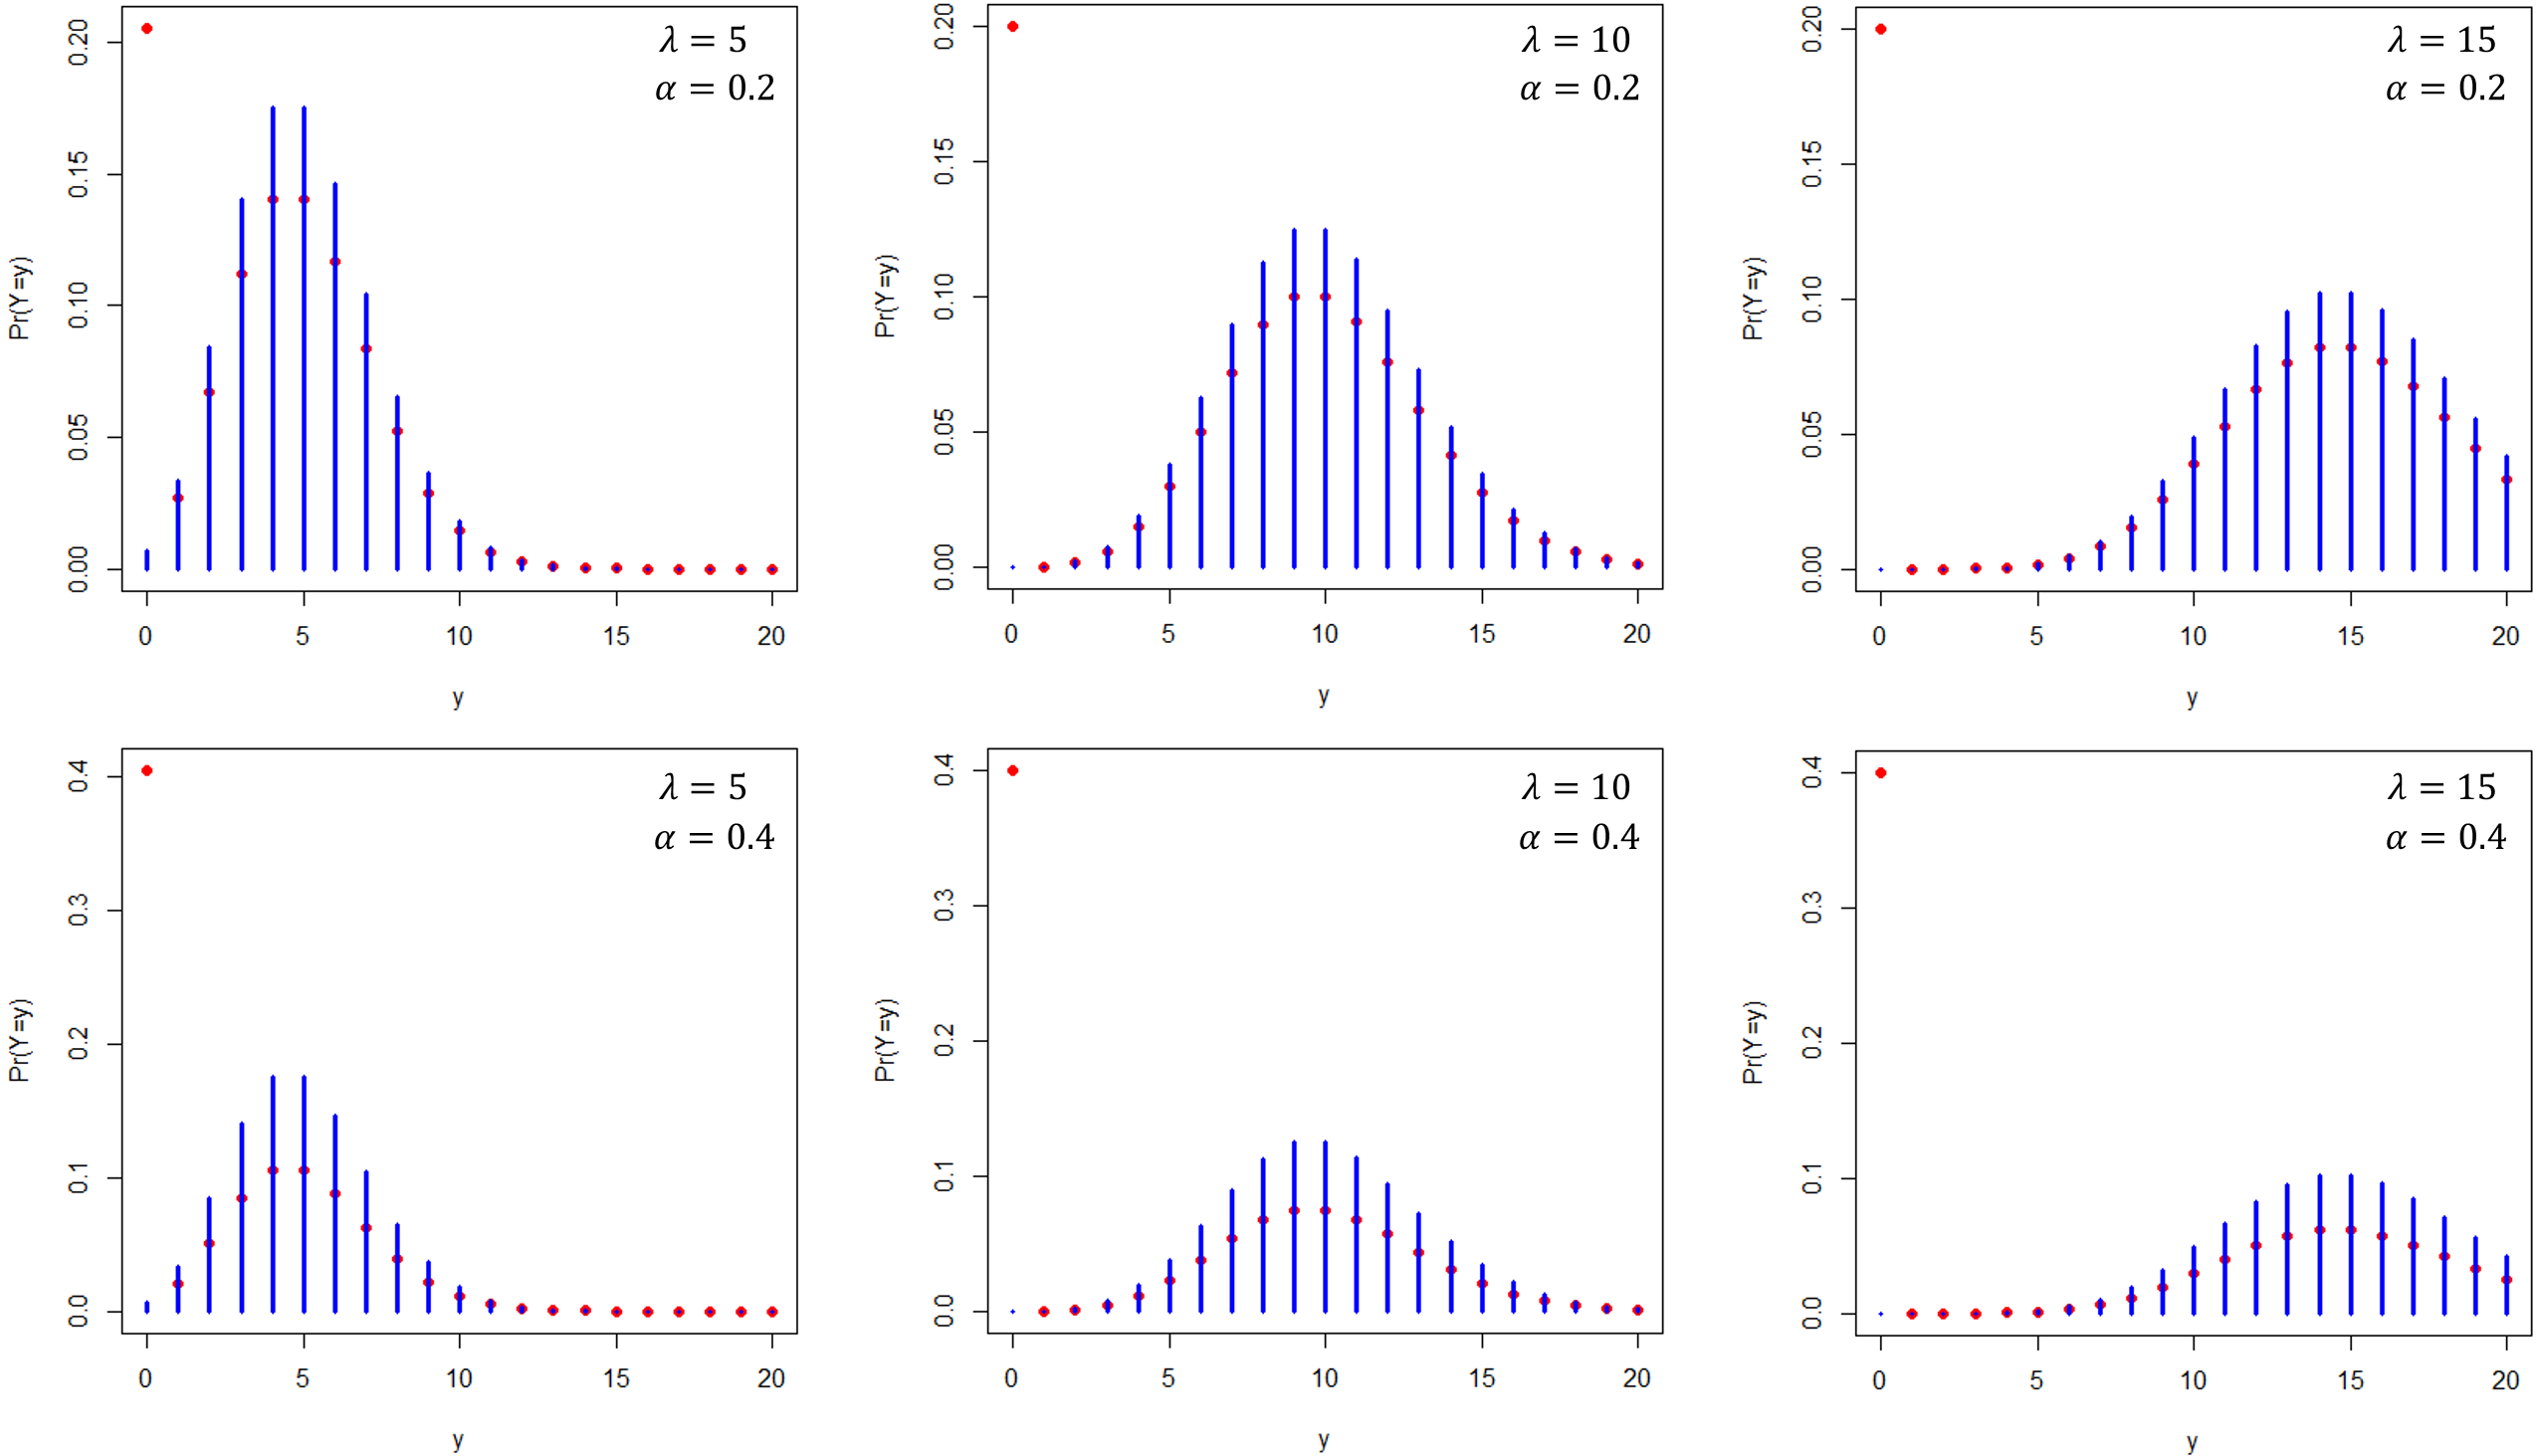
\includegraphics[width=15cm]{ZIP}}
	\caption{Histograms of Poisson (blue) and ZIP (red) PMFs.}\label{F}
\end{figure}








	







\section{Entropy analysis}
In this section, we investigate the entropy measure for an inflated distribution. Let $H(Y)$ be the entropy under the inflated distribution in Eq. \eqref{1} and $H(X)$ be the entropy under the regular distribution.  
In the following theorem, we obtain the entropy $H(Y)$ in terms of $H(X)$. 


\begin{thm}\label{entropy}
	For inflated distribution in Eq. \eqref{1}, the entropy is 
	\begin{align*}
		H(Y)=&(1-\alpha)\bigg(H(X)+\ln(1-\alpha)+\Pr(X=\delta)\ln\frac{(1-\alpha)\Pr(X=\delta)}{\alpha+(1-\alpha)\Pr(X=\delta)}\bigg)\\
		&-\alpha\ln(\alpha+(1-\alpha) \Pr(X=\delta)).	
	\end{align*}
\end{thm}

\begin{proof}
	We have
	\begin{align*}
		H(Y)=&-\sum_{y}\Pr(Y=y)\ln \Pr(Y=y)\\
		=&-\sum_{x}(1-\alpha)\Pr(X=x)\ln((1-\alpha)\Pr(X=x))\\
		&+(1-\alpha)\Pr(X=\delta)\ln((1-\alpha)\Pr(X=\delta))\\
		&-\bigg((\alpha+(1-\alpha)\Pr(X=\delta))\ln(\alpha+(1-\alpha)\Pr(X=\delta))\bigg)\\
		=&-(1-\alpha)\ln(1-\alpha)\sum_{x}\Pr(X=x)+(1-\alpha)H(X)\\
		&+	(1-\alpha)\Pr(X=\delta)\ln((1-\alpha)\Pr(X=\delta))\\
		&-\bigg((\alpha+(1-\alpha)\Pr(X=\delta))\ln(\alpha+(1-\alpha)\Pr(X=\delta))\bigg).
	\end{align*}
	Since $\sum_{x}\Pr(X=x)=1$, therefore the desired result is obtained after rearranging. The theorem is proved. 
\end{proof}

The next theorem compares $H(Y)$ and $H(X)$. 


\begin{thm}
	Consider the inflated distribution in Eq. \eqref{1}. If $H(X)\geq-\ln \Pr(Y=\delta)$, then $H(Y)\leq H(X)$.
\end{thm}

\begin{proof}
	We have $\Pr(Y=\delta)=\alpha+(1-\alpha)\Pr(X=\delta)$. Since $H(X)\geq-\ln \Pr(Y=\delta)$, by Theorem \ref{entropy} we have
	\begin{align*}
		H(Y)=&H(X)-\alpha\bigg(\overbrace{ H(X)+\ln\big(\alpha+(1-\alpha)\Pr(X=\delta)\big)}^{\geq0}\bigg)\\
		&+(1-\alpha)\bigg(\underbrace{\ln(1-\alpha)+\Pr(X=\delta)\ln\frac{(1-\alpha)\Pr(X=\delta)}{\alpha+(1-\alpha)\Pr(X=\delta)}}_{\leq0}\bigg)\leq H(X).
	\end{align*}
	The theorem is proved.
\end{proof}





%\section*{Discussion and Conclusion}   
%The conclusion of the article should be presented in a maximum of 3 or 4 lines.
%\section*{Acknowledgments}   
%If you wish to include acknowledgments, this section should appear before the references.
%%%%%%%%%%%%%%%%%%%%%%%% References %%%%%%%%%%%%%%%%%%%%%%%%%%%%%

\begin{thebibliography}{9}
\bibitem[Shannon (1948)]{Shannon}
Shannon, C.E. (1948). A Mathematical Theory of Communication. \textit{The Bell System Technical Journal} 27, 379--423 and 623--656, July and Oct.

\bibitem[Hartley (1928)]{Hartley}
Hartley, R.V.L. (1928). Transmission of Information. \textit{The Bell System Technical Journal}. 7 (3), 535--563.

\bibitem[Brookes (1956)]{Brookes}
Brookes, B.C. (1956). An Introduction to the Mathematical Theory of Information. \textit{The Mathematical Gazette},  40,  170--180. 

\bibitem[Cohen (1960)]{Cohen}
Cohen, A.C. (1960). Estimating the parameters of a modified Poisson distribution. \textit{Journal of the American Statistical Association} 55, 139--143.

\bibitem[Lambert (1992)]{Lambert}
Lambert, D. (1992). Zero-inflated Poisson regression, with an application to defects in manufacturing. \textit{Technometrics}, 34 (1),  1--14.

\end{thebibliography}
 \end{document}

